\chapter{A Section Name}\chaptermark{Short Version for Top of Page}\label{chap:a section}

% This is an example of how to include published works based on the work in a given chapter. If this is not relevant, please omit.
%%%%%%%%%% Listing Publications at the Start of a Chapter %%%%%%%%%%
% Below are instructions on how to use the environment to list publications. An example of use can be found in a_chapter.tex

% Environment to add text/citations for un/published paper/s at the beginning of the chapter. The environment takes one argument -- specifying how many papers have been PUBLISHED. Use [1] for ONE published paper and any number of unpublished papers, use [2] for TWO OR MORE published papers and any number of unpublished papers, and use [0] for ZERO published papers and ONE OR MORE unpublished papers.

% Usage: 
% \begin{chapter-publications}[2]
% \chappub{Barnes2019saso} % This is the name of the bibtex entry you want to include
% \chappub{Barnes2020BeyondAgents}
% \chapnotpub{Part of this chapter has also been submitted for publication at X.} % This is an unpublished entry. Supply any text as needed
% \end{chapter-publications}

% Alternatively, if not published anywhere but submitted for example:
% \begin{chapter-publications}[0]
% \chapnotpub{The work presented in this chapter has been adapted from work submitted for publication at X.}
% \end{chapter-publications}
%%%%%%%%%%
\begin{chapter-publications}[2]
\chappub{Barnes2019saso}
\chappub{Barnes2020BeyondAgents}
\chapnotpub{Part of the work in this chapter is under review at Journal Name.}
\end{chapter-publications}


\section{Section 1}

\lipsum[1]

		\begin{figure}
    	\centering
    	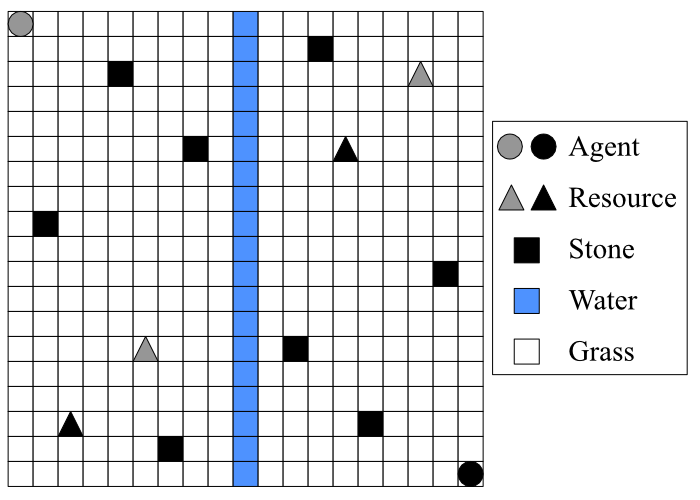
\includegraphics[width=0.75\linewidth]{figures/rcd.png}
    	\caption[The River Crossing Dilemma testbed -- a 2D grid-world environment with a river of Water that agents must cross to retrieve their reward object (Resource).]{The River Crossing Dilemma testbed, which is a 2D grid-world environment. The grey agent (top left) is allocated the two Resources in grey, and the black agent (bottom right) is allocated the two Resources in black; agents cannot interact with Resources that are not allocated to them. Both agents can interact with all other objects. For single-agent environments, the black agent is removed. Figure taken as an example from~\citep{Barnes2021thesis}.}
    	\label{fig: rcd}
	\end{figure}

\lipsum[1]
 
    \begin{figure}
      \centering
      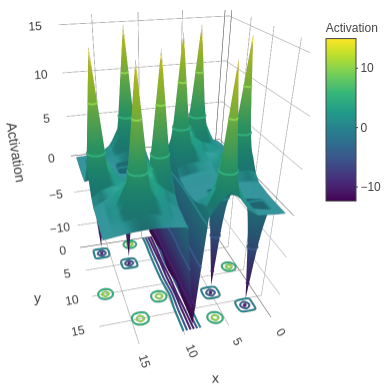
\includegraphics[width=0.5\textwidth]{figures/landscape.png}
      \caption[The reactive network, which generates dynamic activity landscapes that agents use to hill-climb towards their current sub-goals.]{The reactive network generates dynamic activity landscapes with Equation~\ref{eq:shunting equation}, based on the current sub-goals generated by the deliberative network; here, the sub-goals are $[-1,1,-1]$, meaning the agent is attracted to Stones, and avoids Resources and Water. The activity landscape maps to the physical landscape (Figure \ref{fig: rcd}), so agents can hill-climb towards their sub-goals whilst avoiding repulsive objects, by traversing the activity landscape and moving to the adjacent cell with the highest value. Figure taken as an example from~\citep{Barnes2021thesis}.}
      \label{fig: activation landscape}
   \end{figure}
	 
	
	
\section{Another Section}

\lipsum[1] 
    
    An equation here:

    \begin{equation}\label{eq:shunting equation}
        \frac{dx_i}{dt} = -Ax_i + I_i + \sum_{j = 1}^{k} w_{ij}[x_j]^+
        \end{equation}



\section{Using Captioned Sub-Figures}

When using a figure with sub-figures, you can reference individual images such as Figure~\ref{subfig: c}, or the entire figure such as Figure~\ref{fig: some figures}. You can also add \textbf{footnotes}\footnote{Here is an example of a footnote that is formatted correctly, with the correct line spacing and the correct font size.} like this.


    \begin{figure*} 
        \centering
      \subfloat[Caption A \label{subfig: a}
      ]{%
           \includegraphics[width=0.485\linewidth]{example-image-a}}
        \hfill
      \subfloat[Caption B \label{subfig: b}]{%
            \includegraphics[width=0.485\linewidth]{example-image-b}}
        \\
      \subfloat[Caption C \label{subfig: c}]{%
            \includegraphics[width=0.485\linewidth]{example-image-c}}
        \hfill
      \subfloat[Caption D \label{subfig: d}]{%
            \includegraphics[width=0.485\linewidth]{example-image-a}}
        \\
      \subfloat[Caption E \label{subfig: e}]{%
            \includegraphics[width=0.485\linewidth]{example-image-b}}
        \hfill
      \subfloat[Caption F \label{subfig: f}]{%
            \includegraphics[width=0.485\linewidth]{example-image-c}}            
      \caption[A shorter caption. ENSURE ALL FIGURES AND TABLES HAVE A SHORT CAPTION. Do not put references in the short caption, as this forces references to jump to the top of the references list unintentionally.]{A figure containing a number of sub-figures.}
      \label{fig: some figures} 
    \end{figure*}

\section{Using \texttt{siunitx} for Formatting Tables}

The \texttt{siunitx} package is already added to this template, and an example of its use can be found below. This is helpful for formatting numerical data to varying degrees of accuracy, as you paste the entire number into the table and LaTeX will display it to whichever degree of accuracy you specify.

\begin{equation}\label{eq:effect size}
        r = \frac{Z}{\sqrt{N}}
    \end{equation}
    
\begin{table}
	\footnotesize
    	\sisetup{round-mode=figures,round-precision=4,scientific-notation=true,table-format=1.3e-2,table-space-text-post=\sym{*}}
        \def\sym#1{\ifmmode^{#1}\else\(^{#1}\)\fi}
        \def\eff#1{ (#1)}
		\caption[Wilcoxon Signed Rank statistical tests comparing the volatility metrics of agents evolving alone or together, with goal-rational or random action.]{Wilcoxon Signed Rank statistical tests comparing the volatility metrics of agents evolving alone or together, with goal-rational (G) or random (GR) action. $p$-values (to 4 S.F.) are marked with an asterisk (*) if significant ($p < 0.05$). Effect sizes ($r$, to 4 S.F.) are presented with the $z$-score they are calculated from (Equation~\ref{eq:effect size}, $N=100$), and are classed as small (S, $r\geq0.1$), medium (M, $r\geq0.3$), or large (L, $r\geq0.5$) \citep{Cohen1988StatisticalSciences}. Table taken as an example from~\citep{Barnes2021thesis}.}
		\label{tab:g-gr stats}
		\centering
		\begin{tabular}{@{}llSSSS[scientific-notation=false,table-format=-1.4,table-space-text-post=]S[scientific-notation=false,table-format=-1.5,table-space-text-post=\eff{M}]@{}}
			\toprule \multicolumn{1}{c}{\multirow{2}{*}{Metric}} & \multicolumn{1}{c}{\multirow{2}{*}{Experiment}} & \multicolumn{3}{c}{Statistical Test Alternative Hypothesis} & {\multirow{2}{*}{$z$}} & {\multirow{2}{*}{$r$}} \\ \cmidrule(l){3-5}
			\multicolumn{1}{c}{} & \multicolumn{1}{c}{} & \multicolumn{1}{c}{\textit{ $G\neq GR$}} & \multicolumn{1}{c}{ $G < GR$ } & \multicolumn{1}{c}{ $G>GR$ }	\\ \midrule
			\multirow{2}{*}{SDoT}  
			& Alone		& 0.00000001415\sym{*} & 0.000000007077\sym{*} & 1.0 & -5.67 & -0.567~\eff{L} \\
			& Together	& 0.4993 & 0.7515 & 0.2496 & 0.677 & 0.0677 \\ \midrule 
			\multirow{2}{*}{CACoT} 
			& Alone		& 0.000000006814\sym{*} & 0.000000003407\sym{*} & 1.0 & -5.8 & -0.58~\eff{L} \\
			& Together	& 0.00000000000635~\sym{*} & 0.000000000003177~\sym{*} & 1.0 & -6.87 & -0.687~\eff{L} \\ \midrule 
			\multirow{2}{*}{CCoT} 
			& Alone		& 0.000000006146~\sym{*} & 0.00000003073~\sym{*} & 1.0 & -5.81 & -0.581~\eff{L} \\
			& Together	& 0.00000000005557~\sym{*} & 0.00000000002778~\sym{*} & 1.0 & -6.56 & -0.656~\eff{L} \\ \bottomrule
		\end{tabular}
	\end{table}
